\documentclass{sig-alternate-05-2015}

\pdfpagewidth=8.5truein
\pdfpageheight=11truein


\newfont{\mycrnotice}{ptmr8t at 7pt}
\newfont{\myconfname}{ptmri8t at 7pt}
\let\crnotice\mycrnotice%
\let\confname\myconfname%



\setcopyright{acmcopyright}


% DOI
\doi{http://dx.doi.org/xx.xxxx/xxxxxxx.xxxxxxx}

% ISBN
\isbn{978-1-4503-4486-9/17/04}

%Conference
%\conferenceinfo{PLDI '13}{June 16--19, 2013, Seattle, WA, USA}

\acmPrice{\$15.00}

%
% --- Author Metadata here ---
\conferenceinfo{SAC'17,}{ April 3-7, 2017, Marrakesh, Morocco}
\CopyrightYear{2017} % Allows default copyright year (20XX) to be over-ridden - IF NEED BE.
%\crdata{0-12345-67-8/90/01}  % Allows default copyright data (0-89791-88-6/97/05) to be over-ridden - IF NEED BE.
% --- End of Author Metadata ---




%\usepackage{makeidx}  % allows for index generation
\usepackage{cite}
\usepackage{color}
\usepackage{balance}
%\usepackage{times}
\usepackage{url}
\urlstyle{same} % formats footnotes
%\usepackage{xcolor}
\usepackage{pgfplots} %% Image png
\usepackage{soul} % highlighting
%\usepackage{multirow}
%\usetikzlibrary{patterns} %% Used for bar charts
%\usepackage{float} %% Used for side by side minipages
%\usepackage{multirow}
%\usepackage{subfigure} % Needed for showing charts side by side

%\usepackage{amssymb}% Checkmark
\usepackage{caption} % Bar chart
\usetikzlibrary{patterns} % Bar chart
\usepackage{amssymb} % \Checkmark
\usetikzlibrary{patterns} % Bar chart
\usetikzlibrary{fit, } %% Used for putting dotted box


%%
%\usepackage{tikz}
%\usepackage{caption}
%\usepackage{soul} % Used for highlighting % \hl{this is some highlighted text}
%\usepackage{times} % Used for formatting formatting url footnotes
%\urlstyle{same} % Used for formatting formatting url footnotes
%\usepackage[binary-units=true]{siunitx}




% Define flow chart styles
\tikzstyle{decision} = [diamond, draw, fill=blue!20,
    text width=15em, text badly centered, node distance=3cm, inner sep=0pt]
\tikzstyle{block} = [rectangle, draw, fill=blue!20,
    text width=15em, text centered, rounded corners, minimum height=4em]
\tikzstyle{line} = [draw, -latex']

\usetikzlibrary{shapes,arrows, positioning} % Needed for analysis diagram



% Anonymous
\newif\ifisnopii
%\isnopiitrue % change to true/false to remove personally identifiable information (pii)
\isnopiifalse % change to true/false to remove personally identifiable information (pii)




\newcommand{\todo}[1]{\textcolor{cyan}{\textbf{[#1]}}}
\newcommand{\dan}[1]{\textcolor{blue}{{\it [Dan says: #1]}}}
\newcommand{\yasmine}[1]{\textcolor{blue}{{\it [Yasmine says: #1]}}}
\newcommand{\sam}[1]{\textcolor{blue}{{\it [Sam says: #1]}}}

\makeatletter
\renewcommand\@biblabel[1]{}
\makeatother


\begin{document}


%\title{Permission Usage in Open Source Android Apps}
%\title{Permissions in Open Source Android Apps: Who adds them? When and Why?}
\title{Most Recent Version is in Overleaf: Who Added that Permission to My Android App? An Analysis of Developer Permission Changes in Open Source Android Apps.}


\numberofauthors{1} %  in this sample file, there are a *total*
% of EIGHT authors. SIX appear on the 'first-page' (for formatting
% reasons) and the remaining two appear in the \additionalauthors section.
%
\ifisnopii % turn on/off pii
\author{
%
% 1st. author\
\alignauthor
Daniel~E.~Krutz YASMINE~\&~Samuel~A.~Malachowsky\\ 	
	\affaddr{Software Engineering Department}\\
       \affaddr{Rochester Institute of Technology}\\
       \affaddr{1 Lomb Memorial Drive}\\
       \affaddr{Rochester, NY, USA} \\
       \email{\{dxkvse, samvse\}@rit.edu}
       \alignauthor
} % Must not be a space above this

\else % turn on/off pii
\author{
%
% 1st. author
\alignauthor
xxxxxxxxxxxxxxx\\ 	
	\affaddr{xxxxxxxxx}\\
       \affaddr{xxxxxxxxx}\\
%       \affaddr{xxxxxxxxx}\\
       \affaddr{xxxxxxxxx, xx, xxx} \\
       \email{xxxxxx@xxxxx.xxx}
       \alignauthor
} % Must not be a space above this
\fi % end turn on/off pii

\maketitle


\begin{abstract}

Android applications (apps) rely on a permission-based model to carry out core functionality. Appropriate permission usage is imperative for ensuring proper device security and protecting the user's desired privacy levels. But who is making the important decisions of which permissions the app should request? Are they experienced developers with the appropriate project knowledge to make such important decisions, or are these crucial choices being made by those will only minor amounts of project experience? When are these permission decisions being made in the app's development lifecycle? Are they added at the beginning of the project, or are they steadily added throughout the lifecycle of the app?

In this work, we examine a large set of open source Android version control repositories to better understand when, why, and who is adding permissions. Our primary findings include: I) There is no significant correlation between the ratio of permissions-based commits and overall project commits by a developer. Our data indicates that developers with a low number of overall project commits make a disproportionately high number of permissions-related commits. II) There is no significant correlation between an app's user rating and the ratio of permissions-altering commits to overall commits. III) Permissions are added at a reasonably consistent rate throughout the software development process. 


%In the following work we further describe our analysis and findings, along with presenting a publicly available data set from our work which other researchers may use in their work.

%\todo{Add yasmine?}
%\todo{just as likely to make permissions and substractions}
%\todo{Add more of an analysis to the paper. Why do people care? Why is this work important? What problems does it solve?}


%%% Also look to see who is removing the overprivs. Are certain people more likely to remove overprivs?

\end{abstract}
% \keywords{Android Permissions, Mining Software Repositories, Software Evolution}



\section{Introduction}

Android is the world's most popular mobile OS~\cite{OSMarketShare_URL} with over 1.8 million apps available from Google Play alone~\cite{statistica_url}. A cornerstone of Android security is its usage of permissions. Android apps do not have any default permissions associated with it. A developer must explicitly state the permissions an app must request, while the end user must accept any requested `dangerous' permissions, some of which include the ability to read SMS messages, record audio through the phone's microphone, and access the user's location~\cite{AndroidSystemPermissions_URL}.

The decision of which permissions an app should have access to should not be taken lightly since they carry a variety of possible security and functional implications. Some of which include under \& over-permissions, increased app susceptibility to malware and unwanted data leakage to ad libraries~\cite{Felt:2011:APD:2046707.2046779, Grace:2012:UEA:2185448.2185464}. But who is making these important decisions about the permissions an app should request? Who is deciding what gateways the app should request to make into our digital lives? Developers often rely upon user ratings of their software in the app stores in order to remain successful~\cite{Khalid_Mei_Examinging, al2015app}. Is there any correlation between what developer project experience levels are making permission-based decisions, and this all important user rating? To more properly address these permissions-based issues, we need to understand more about permissions in the app development process. In the following work, we describe our examination of  open source Android app repositories in order to better understand how permissions fit into the development process. Our work is guided by the following research questions:



%% Mention why these results are important

\noindent
\textbf{RQ1:}~\emph{What is the correlation strength between the overall number of commits by a developer, and permission-based commits?} Our work indicates that developers with a low number of project commits make a disproportionately high number of permissions-based project decisions. This indicates that developers with small amounts of project experience are making a disproportionately high number of project based decisions.

%  and that there is no significant correlation between the number of project commits, and permissions-related project commits

\noindent
\textbf{RQ2:}~\emph{Is there a correlation between the ratio of developer permission-based commits to overall project commits, and user ratings?} We found virtually no relationship between the ratio of developer permission-based commits to overall project commits, and user ratings. This indicates that there is no strong correlation between who is adding the permissions to an app, and its user rating.


\noindent
\textbf{RQ3:}~\emph{At what development stages are permissions being added to Android projects?} We found that permissions are added at a fairly consistent level throughout the development life cycle of an app. This indicates that permission-based decisions are steadily made throughout the development of the app.

%, but often encounter spurts in permission additions at various stages.

\newpage
The rest of the paper is organized as follows: In Section~\ref{sec: relatedworks} we discusses related work and Section~\ref{sec: androidapps} describes the permission structure of Android apps. Section~\ref{sec: collection} presents our collection and analysis process, while Section~\ref{sec: evaluation} addresses our research questions. Section~\ref{sec: publicdata} discusses our public data set and tool which we hope can be used to assist others in their research. Section~\ref{sec: futurework} discusses future work to be conducted in this area, while Section~\ref{sec: conclusion} concludes our work.


\section{Related Work}
\label{sec: relatedworks}

There has been a substantial amount of work in understanding why Android permissions are inappropriately used, and the negative implications misuse carries.  Grace et al.\cite{Grace:2012:UEA:2185448.2185464} conducted work on permissions probing, which is when a 3rd party component attempts to use a permission in the hope that the attached app has requested it from the user. If the attached app has requested a permission, then the component will also have access to that permission as well. This is often done to collect, and transmit potentially sensitive information which should not be normally available to the 3rd party component. They found that more than half of all ad libraries try to probe for open permissions. This could often be the cause of an under-permission in an app since the ad library will try to use a permission which the developer did not request.

Stevens~\emph{et al.}\cite{6624000} analyzed 10,000 free Android apps and found a strong sub-linear relationship between the popularity of a permission and the frequency of its misuse. They found that developers were more likely to misuse a permission when they did not understand it, and that the popularity of a permission is strongly associated with its misuse. A powerful method of avoiding permission misuse is through developer education and community support. Krutz~\emph{et al.}\cite{krutz2015FDroid} created a public dataset of over 1,100 Android apps from the F-Droid\footnote{https://f-droid.org/} repository. This research focused more on the life cycle of the apps and how each iteration of the app evolved with every version control commit and placed more of an emphasis on analyzing the app from other quality perspectives.


% Research has been conducted in analyzing the effects of permissions on the user's perception of the app. Egelman et al.\cite{Egelman12choicearchitecture} found that approximately 25\% of users were typically willing to pay a premium in order to use the same application, but with fewer permissions. Contrary to these findings, other research has argued that users typically pay little attention to permissions when installing an app, and often do not understand or care about the precise functionality for most of the granted permissions~\cite{Felt:2012:APU:2335356.2335360, Kelley:2012:CPI:2426020.2426027}.



Previous works have analyzed effects of permissions on the user's perception of the app. Lin et al.\cite{Lin:2012:EPU:2370216.2370290} examined user comfort levels when using permissions they did not fully understand, or when they did not comprehend why the app needed the permission. They found that users generally felt uncomfortable and may even delete applications when they did not understand why it requested a permission they deemed unnecessary. Egelman et al.\cite{Egelman12choicearchitecture} found that approximately 25\% of users were typically willing to pay a premium in order to use the same application, but with fewer permissions, while about 80\% of users would be willing to allow their apps more permissions to receive targeted advertisements if it would save them .99 cents on the purchase of the app. Contrary to these findings, other research has argued that users typically pay little attention to permissions when installing an app, and often do not understand or care about the precise functionality for most of the granted permissions~\cite{Felt:2012:APU:2335356.2335360}. Kelley et al. \cite{Kelley:2012:CPI:2426020.2426027} conducted semi-structured interviews with Android users, and found that users paid limited attention to permission screens, and had poor understanding of what these permissions implied.%\dan{shorten a bit?} % I'm not sure all of this information is needed


App ratings have demonstrated their importance in other areas of research as well. Harman et al.\cite{6224306} found a strong correlation between the rating and the number of app downloads. Linares-Vasquez et al.\cite{Linares-Vasquez:2013:ACF:2491411.2491428} found that fault-proneness of the APIs used by the apps negatively impacts their user ratings. Khalid et al.\cite{Khalid_Mei_Examinging} examined 10,000 apps using FindBugs and found that warnings such as~\lq Bad Practice\rq, ~\lq Internationalization\rq, and~\lq Performance\rq  categories are typically found in low-rated apps. They found that app developers could use static analysis tools, such as FindBugs, to repair issues before users complained about these problems. Even though we too use ratings as an evaluation measure, unlike earlier works we look at permission and security risks. % I'm not sure all of this information is needed



% \todo{other papers have mentioned that the app permission rate is steadily growing} % Check the MPerm paper for this citation


\section{Android Permissions}
\label{sec: androidapps}

Android apps require specific permissions to carry out specific functionality. A primary goal of this system is the adherence to the \emph{principle of least privilege} or granting an app the least amount of privilege that it needs to properly function. This is intended to not only limit the access an app has to unintended permissions, but limit the effects that malware may have on a device. For example, in order for an app to read SMS messages, it must request the \texttt{READ\_SMS} permission, and to use the camera the app would request the \texttt{CAMERA} permission. The~\emph{AndroidManifest.xml} file contains all requested permissions for an app. While many permissions are considered to be less risky or \emph{Normal} permissions, others carry significantly more potentially hazardous risks and are known as \emph{Dangerous} permissions. Users must explicitly allow the app to make use of these more threatening permissions. Deciding on the permissions an app should request is considered to be one of the most sensitive activities undertaken during app development due to the potential security risks~\cite{Felt:2011:APD:2046707.2046779, 5482589} and possible negative effects on the user's perception of the app~\cite{Egelman12choicearchitecture}. In our analysis, we recorded both Normal and Dangerous permissions which were requested by the app.

Developers frequently make permissions based mistakes by adding too many, or too few permissions to an app. This may be caused by a variety of factors including a lack of permissions based on knowledge by the developers~\cite{6624000}. Unfortunately, there is no permissions enforcement mechanisms in Google Play, which frequently gives developers too much freedom when posting apps to the Google Play store~\cite{Barrera:2012:UIA:2381934.2381949}. In this study, we use the term \emph{over-permission} to describe a permission setting that grants more than what a developer needs for the task. Likewise, an \emph{under-permission} is when an app was not given all the permissions that it needs to properly function as intended.


 %is a setting for which the app could fail because it was not given the proper permissions. If not properly handled, an application, could throw a~\emph{SecurityException} when it attempts to perform an operation which it does not have permission to conduct.


%Android apps operate under a permission-based system where an app requires specific permissions to carry out specific functionality.
%Unfortunately, developers often request more permissions than they actually need, as there is no built in verification system to ensure that they are only requesting the permissions their application actually uses~\cite{Felt:2011:APD:2046707.2046779}.


%% Maybe add back in if space allows
%Over-permissions are considered security risks since they do not adhere to the principle of least privilege and may unnecessarily increase an app's attack surface. Under-permissions are considered quality risks, with a possible indication of permission probing. The primary difference between requested permissions and over-permissions is that requested permissions are merely those that the app asks to use, and does not take into consideration if the app actually needs them or not. While largely a quality concern, under-permissions can represent a possible security concern as well. One example of this is when permissions are, unknowingly to the developer, misused in a variety of ways by 3rd party libraries or even by associated ad networks which may collect and transmit potentially sensitive user data~\cite{Grace:2012:UEA:2185448.2185464}. Under-permissions essentially leave a door open for other system operations, malicious or not, to use.


% There is a strong correlation between the rating and the number of app downloads \cite{6224306}

%% Can add more to this from the material in the other papers


\section{Data Collection and Analysis}
\label{sec: collection}

%Our dataset was built in two primary phases: the data collection process which included gathering source code and version control information from the F-Droid repository, and then analyzing the this information using a custom built tool, oSARA.

%\hl{In order to analyze the collected repositories, we created a tool known as the Open Source Android Repository Analyzer (oSARA)}. Using this tool,

Following a process similar to one defined by Krutz et al.\cite{krutz2015FDroid}, our first step was to collect open source Android repositories from F-Droid, which hosts over 1,100 open source Android apps. We collected the complete git repositories for each app, which contains all version control information about each project. In order to analyze the collected repositories, we created a tool known as `the Open Source Android Repository Analyzer (oSARA). Using this tool, we extracted version control commit information such as when the commit was made and who the committer was. The committed version of the AndroidManifest.xml file was also extracted from from the repositories, and all metadata was stored in a SQLite database. Using this information, we were able to correlate the altered Android permissions with a specific commit in the version control repository. We then calculated the Developer's Commit Ratio (DCR) for each app, which is defined as: DCR = $(\frac{Individual Author Commits}{Total App Commits})$. For each committed AndroidManifest.xml file that contained altered permissions, we recorded this DCR value. In this analysis, we only examined the master branch for each git repository, and only considered apps with at least 2 committers and at least 10 commit updates to the AndroidManifest.xml file. This left us with a total of 481 apps and a total of 13,036 manifest commits.



% View to get the 481 apps
% select AppID, count (AppID) as AppCount from android_manifest_commitinfo group by appID


%% No way to ensure that single developers are not using muliple accounts

%% User Ratings
We then determined the average Google Play user rating for each of the collected apps, which we found by matching the retrieved package and app name to the corresponding app in Google Play. We did not create associations when we did not find matches for both the package and app name, and excluded this information from our analysis. We also excluded apps with less than 25 user reviews, leading to a total of 96 apps. This sample size is larger or similar in size to other studies which have examined user feedback in Android apps~\cite{Khalid:2014:PDT:2635868.2635909, Gui:2015:TAH:2818754.2818769}. An overview of the data collection and analysis process is shown in Figure~\ref{fig:analysisprocess}.


    \tikzstyle{line} = [draw, -latex']

    \tikzstyle{block} = [rectangle, draw, fill=white!20,
    text width=5em, text centered, rounded corners, node distance=2.2cm, minimum height=4em]

	\tikzstyle{database}= [fill=blue!20, cylinder, shape border rotate=90, draw,minimum height=2.2cm,minimum width=1.55cm]

	\begin{figure}[h!]
	\begin{center}
% \resizebox {\columnwidth} {!} {  %% Makes the image too big
    \resizebox{.45\textwidth}{!}{
	\begin{tikzpicture}[node distance = 2cm, auto,   hhilit/.style={draw=black, thick, densely dotted,label=oSARA Tool,inner xsep=.3em,inner ysep=.7em},]
    % Place nodes
     		\node [database] (init) {F-Droid};
     		\node [block, right of=init] (jar) {Collect Repositories};
     		\node [block, right of=jar] (java) {Analyze Repositories};
     		\node [block, right of=java] (R) {Data Analysis};
 %           \node [block, right of=R] (sqlite) {SQLite DB};


   \node[hhilit, fit=(java) (R)] {};



            \path [line] (init) -- node {}(jar);
     		\path [line] (jar) -- node {}(java);
     		\path [line] (java) -- node {}(R);
%            \path [line] (R) -- node {}(sqlite);

	\end{tikzpicture}
%	}
}
	\end{center}
	\caption{App Repository Collection and Analysis Process}
	\label{fig:analysisprocess}
	\end{figure}





% \vspace{-8mm}



\section{Evaluation}
\label{sec: evaluation}

% Our primary research questions will be answered in the following section.

%\todo{create a scatter plot of the collected data}



Using the collected data, we were then able to address our research questions. \\

\noindent
\textbf{RQ1: What is the correlation strength between the overall number of commits by a developer, and permission-based commits?} %\emph{We found that developers with low project commit ratios make a disproportionately high number of permissions-based project decisions and that there is no correlation between the number of project commits, and permission related project commits.}

%\todo{create a scatter plot for this}

Our first goal was to calculate the ratio of a developer's permission-based commits to overall project commits. Understanding the project experience levels of who is making permissions-related project decisions is important since permissions often negatively affect a user's perception of the app~\cite{Egelman12choicearchitecture} and carry numerous security related risks~\cite{Felt:2011:APD:2046707.2046779, 5482589}. Using oSARA, we recorded the developer's DCR score for each added or removed permission in the app's commit history, which provided us with a ratio of a developer's permissions-related commits to overall project commits. In our analysis, we were careful to count only altered permissions in an app's commit history. If a developer did not change the app's requested permissions, this commit was not included in our permissions-related analysis since it did not include a permissions-related alteration. However, this commit would be included in our count of the overall developer commits since it did involve other alterations to the project. We recorded the average DCR mean, mode, median, and standard deviation for all analyzed apps. The results of this analysis is shown in Table~\ref{Table:percentageCommitPermssion}.


\begin{table}[h]
\begin{center}
\caption{Developer DCR Statistics}
\label{Table:percentageCommitPermssion}
 \begin{tabular}{ | l | c | c | c | c | } \hline

  \bfseries Permission Action & \bfseries Mean & \bfseries Mode & \bfseries Median & \bfseries Std  \\ \hline

    Add & .52 & .84 & .45 & .333 \\ \hline
    Remove & .524 & .84 & .5 & .335 \\ \hline \hline
    Total & 0.521 & 0.84 & .5 & .334 \\ \hline
	
  \end{tabular}
  \end{center}
\end{table}


%% The data is now skewed and is centered around .5, but it is widely distributed
%All
%Mean	0.521483898
%Mode	0.84
%Median	0.5
%Std	0.333794422
%Range	1
%
%+
%Mean	0.519277382
%Mode	0.84
%Median	0.45
%Std	0.332817837
%Range	1
%
%
%-
%Mean	0.523728766
%Mode	0.84
%Median	0.5
%Std	0.334779493
%Range	1




%%% low presenters are responsabile for X number of the commits

Although the mean of the DCR values are centered around .52, the large standard deviation of .33 demonstrates a significant variation of the DCR levels among all of the developers. In order to better understand this large range, we next examined the DCR level of committers at a much more granular level. Our first step was to group all developers into five groups based on their percentage of commits they were responsible for in an individual project. For each of these groups, we determined the average number of permissions both added and removed  for each developer in this group. The results of this analysis is shown in Figure~\ref{fig:permissionRanges}.


% Table~\ref{Table:permissionRanges}.


 %%% Get all the commits for these users, not just their permission based commits
 %%     Wouldn't it just be lower there?


% \begin{table}[h]
%\begin{center}
%\caption{Developer Commit Ranges\todo{bar chart}}
%\label{Table:permissionRanges}
% \begin{tabular}{ | c | c | } \hline
%
%  \bfseries \% of Project Commits & \bfseries \% of Permissions Based Alterations \\ \hline
%
%    0-.19 & 24    \\ \hline
%    .2-.39 & 11    \\ \hline
%    .4-.59 & 20    \\ \hline
%    .6-.79 & 14   \\ \hline
%    .8-1.0 & 31    \\ \hline
%
%  \end{tabular}
%  \end{center}
%\end{table}




%\definecolor{bblue}{HTML}{4F81BD}
%\definecolor{rred}{HTML}{C0504D}
%\definecolor{ggreen}{HTML}{9BBB59}
%\definecolor{ggrey}{HTML}{707070}
%
%
%\begin{center}
%\begin{tabular}{@{}lp{2cm}}
%%\resizebox {\columnwidth} {!} {
% % \resizebox{.8\textwidth}{!}{
%% \scalebox{.9}[0.85]{ %Width, Height
%\scalebox{1.1}[.9]{ %Width, Height
%\begin{tikzpicture}
%    \begin{axis}[
%        width  = .50*\textwidth,
%        height = 8cm,
%legend style={at={(0.47,0.3)},anchor=north},
%        major x tick style = transparent,
%        ybar,
%%        bar width=10pt,
%        bar width=18pt,
%        ymajorgrids = true,
%	xlabel={Developer Commit Group by Percentage of Commits},
%	ylabel = {Average Developer DCR \%},
%        symbolic x coords={0-.19,.2-.39, .4-.59, .6-.79, .8-1},
%        xtick = data,
%        scaled y ticks = false,
%    ]
%
%       \addplot[style={ggreen,pattern=north east lines,mark=none}, postaction={}] % Precision
%           coordinates {(0-.19, 24) (.2-.39,11)(.4-.59,20)(.6-.79,14)(.8-1,31)};
%
%    \end{axis}
%
%\end{tikzpicture}
%}
%\end{tabular}
%  \captionof{figure}{Developer Commit Ranges\todo{add bar items}}
%\label{fig:permissionRanges}
%\end{center}









\definecolor{bblue}{HTML}{4F81BD}
\definecolor{rred}{HTML}{C0504D}
\definecolor{ggreen}{HTML}{9BBB59}
\definecolor{ggrey}{HTML}{707070}


\begin{center}
\begin{tabular}{@{}lp{2cm}}
%\resizebox {\columnwidth} {!} {
 % \resizebox{.8\textwidth}{!}{
% \scalebox{.9}[0.85]{ %Width, Height
\scalebox{.95}[.95]{ %Width, Height
 \begin{tikzpicture}
    \begin{axis}[
        ybar stacked,
      legend style={at={(0.23,0.8)},anchor=west},
        bar width=14pt,
%        axis lines*=middle,
        xlabel={Developer Commit Group by Percentage of Commits},
	ylabel = {Average Developer DCR \%},
        symbolic x coords={0-.19,.2-.39, .4-.59, .6-.79, .8-1},
        axis on top=false,
        xtick=data,
        enlargelimits=0.2 %% Add padding to the right and left of the bars
        %enlarge y limits=0.2,
       % after end axis/.code={
%            \node at ({rel axis cs:0,0}|-{axis cs:0,0}) [anchor=east] {0};
%        }
    ]
      \addplot[
        fill=ggreen,
        draw=none,
%        bar shift=8pt,
        mark options={
            gray,
            thick,
            dashed
        },
        mark=waterfall bridge
        %% Added permissions
      ] coordinates { (0-.19, 12) (.2-.39, 05) (.4-.59,11) (.6-.79,07) (.8-1,15) };
      \addplot[
        fill=ggrey,
        draw=none,
 %       bar shift=8pt
        %% Removed permissions
      ] coordinates { (0-.19,12) (.2-.39,06) (.4-.59,09) (.6-.79,07) (.8-1,16)};
      \legend{Added Permissions, Removed Permissions}
    \end{axis}
  \end{tikzpicture}
}
\end{tabular}
  \captionof{figure}{Developer Commit Ranges}
\label{fig:permissionRanges}
\end{center}




%This demonstrates and that over 55\% of all permissions based commits are being made by these two groups.




% Find a project example where this was a problem, maybe even not a problem



This demonstrates that a surprisingly large number of authors with low amounts of project based commits performed a large number of permission-related commits. For example, authors who performed less than 20\% of an app's total commits performed 24\% of a project's permission-related commits. Permissions-related commits for authors who had significantly more project related commits was higher, but still not proportional with the number of overall project commits. We also found that developers in each group had approximately the same likelihood of adding or removing permissions.


% The data collected from the static analysis tools along with user ratings data was analyzed using standard libraries, such as the {\it stats} library in R.


We next used the Spearmen, Kendall and Pearson correlation metrics to determine the correlation strength between a developer's total project commits, and permission-based commits. The results of our analysis is shown in Table~\ref{Table:commitownership}. When using these correlation metrics, the correlation coefficient will vary between -1 and +1. As the value of the coefficient approaches $\pm$1, there is more of a monotonic, or perfect degree of association between the evaluated values. The relationship between the evaluated values becomes weaker as the correlation coefficient approaches 0. Our findings demonstrate an extremely weak association between the total number of application commits, and permissions-related commits. This further indicates that developers with a low number of project commits were making a disproportionally high number of permissions-related commits.

\begin{table}[h]
\begin{center}
\caption{Correlation of Total Commits and permission-based Commits}
\label{Table:commitownership}


    \begin{tabular}{ | c | c | c | } \hline

    \bfseries ~~~~Spearman~~~~ & \bfseries ~~~~Kendall~~~~ & \bfseries ~~~~Pearson~~~~  \\ \hline \hline
    0.044 & 0.025 & 0.067 \\ \hline
  \end{tabular}

  \end{center}
\end{table}


%\todo{so what? Why are developers doing this?}
%- Maybe find specific cases to examine



% Possible examples
%	A low committer makes a permission mistake that someone else fixes... look for commit comments
%	





%%% So what to all of this
%	Are there problems with the permissions that less committers added in?
%		Are the permissions less committed authors more likely to be removed?
%		Are they more likely to be overprivs
%		What other problems can permissions have?








%%% Next show the chart with the ownership vs. Permission info "growthrate "





%\noindent
%\textbf{Discussion:} % implications

\vspace{5mm}
\noindent
\textbf{Analysis:}
The implications for these results are important since the proper use of permissions is crucial for a variety of security and functional reasons~\cite{Felt:2011:APD:2046707.2046779, 5482589, Egelman12choicearchitecture}. A key question is why developers with such a low number of overall project commits are making a disproportionately high number of permissions-based decisions. There are several possible explanations for this which should be further explored. One possibility is that developers with less project commits will have less overall project knowledge, and will mistakenly believe that permissions should be added or removed from the project. A contrarian view would suggest that `permission experts' perform a large number of permission-related changes to apps, but do not make a significant number of other alterations.  %\dan{add to this}




%We next checked to see if there were any positive or negative ramifications of developers with a low overall DCR score making a disproportionately high number of permissions related commit mistakes. Using Stowaway~\cite{Felt:2011:APD:2046707.2046779}, a popular permissions gap detection tool, we compared the rate of under and over-permissions introduced by high and low project committers. In order to create a group of low-committers, and high-committers for comparison, we next sorted developers based on their DCR scores, using a process similar to that Tian et al\cite{tian2015characteristics}. To create a set of low-committers apps, we selected the bottom 10\% of committers with the lowest DCR scores, while our high-committers apps were comprised of the top 10\% DCR scores. This created a set of 64 committers in both our low-rated and high-rated data sets.



%The median rating of the low-rated apps is 3.2, while it is 4.6 for high-rated apps. %The median number of downloads for low-rated apps is 10,000 and is 100,000 for high-rated apps.\todo{fix} %% Not sure if this should be included


%%% Look at OverprivOwnershop.xlsx tabs top10 & bottom 10
%		Query: OverPrivsAndOwner_view




%%% stuck

%%%% Repeating appID 663.
% No joins = 642

%--    drop view OverPrivsAndOwner_view;
%--    create view OverPrivsAndOwner_view as
%    select * --uv.AppID, uv.AppName, uv.Author, uv.Email, uv.AuthorCount, uv.TotalCount, uv.PermOwner--,OPrivCount, UPrivCount
%    from UserPermUpdate_view uv
%	
%	
%    left join (select count(PermName) as OPrivCount, ouv.Author, ouv.AppName, ouv.adAppID, ouv.amAppiD, build_number, email
%    from OPrivs_To_UserPrivs_view ouv
%    inner join (select max(build_Number) as maxBuild, adAppID from OPrivs_To_UserPrivs_view group by adAppID) mb on mb.adAppID = ouv.adAppID and mb.maxBuild=ouv.build_number
%--    group by ouv.adAppID, Author) ouv2 on ouv2.AppName = uv.AppName and ouv2.Email = uv.Email
%	group by ouv.adAppID, Author) ouv2 on uv.AppID = ouv2.amAppiD and ouv2.Email = uv.Email
%	
%	/*
%	left join (select count(PermName) as UPrivCount, upc.Author, upc.AppName, upc.adAppID, upc.amAppiD, build_number, email
%    from UPrivs_To_UserPrivs_view upc--ouv
%    inner join (select max(build_Number) as maxBuild, adAppID from UPrivs_To_UserPrivs_view group by adAppID) mb on mb.adAppID = upc.adAppID and mb.maxBuild=upc.build_number
%    group by upc.adAppID, Author) ouv3 on ouv3.AppName = uv.AppName and ouv3.Email = uv.Email
%	*/
%    order by appID--, author, Email
%	
	



%Our null hypothesis is that there is no difference in the distribution of the misused permission metrics between the low and high-rated committers. Our alternate hypothesis is that low and high-rated committers have different distributions for each of the permission related metrics. We use the one tailed Mann Whitney U (MWU) test for the hypothesis testing, since it is non-parametric and we can find out if the low-rated apps indeed have higher or lower values for each of the security metrics. In our analysis, we used an $\alpha$-value of .05 to determine if the null hypothesis can be rejected or not. We represent p > 0.05 with a `-' in our results. We next measured the strength of association between our collected security metrics using the Spearman rho correlation metric. The results of this analysis are shown in Table~\ref{table:appCorrelationMetrics}.

% We used the Spearman rho and Kendall correlation metrics to determine if there was a correlation between quality and security. Using these correlation metrics, we evaluated the relationship strength of quality (Coding Standards Defects \& Jlint Errors) and security (Androrisk \& over-permissions). The results of this analysis are shown in Table~\ref{table:appCorrelationMetrics}.



%%%%% Future work: Are developers with a higher DCR score more likely to remove overprivs? This analysis was not possible for us since we only had the most recent version of the app, and coul --- Check to make sure that this is consistent with the rest of the paper


%%% Do some developers make mistakes on specific permissions




% \checkmark


%%% If this doesn't work, think of a different way it can be broken up


%\begin{table*}[th]
%\renewcommand{\arraystretch}{1.5}
%\centering
%\caption{MWU Analysis Results}
%\begin{tabular}{|l|l|c|c|l|}
%    \hline
%    \multirow{3}{*}{\textbf{Category}} & \multirow{3}{*}{\textbf{Analysis}} & \multicolumn{3}{c|}{\textbf{MWU}}                                            \\ \cline{3-5}
%                                       &     & \multicolumn{2}{c|}{\textbf{Greater In}} & \multirow{2}{*}{\textbf{p-value}} \\ \cline{3-4}  &      & \textbf{Low Committers} & \textbf{High Commtters} &                                   \\ \hline \hline
%    \multirow{4}{*}{All}               & Permissions                        & -                  & -                   & X                        \\ \cline{2-5}
%                                       & Over-Permissions                   &                    &    & \textbf{X}               \\ \cline{2-5}
%                                       & Under-Permissions                  &                    &          & \textbf{X}               \\ \hline %\hline
%                                   %    & Androrisk Score                    &                    &          & \textbf{X}               \\ \hline \hline
%
%
%
%\end{tabular}
%\label{table:appCorrelationMetrics}
%\end{table*}





%%% Next, go into





%\todo{....Add more analysis.....} % Do a high & low analysis
%^%%% Take the top 10 % and bottom 10% of developers and do a MWU to see if one group is more likely to create overprivs








% using a process similar to that Tian et al\cite{tian2015characteristics}



%%%% Create table with MWU results







%\todo{----------------- \\}




%%%%%%%%%%%%%%%%%%%%%%%%%%%%%%%%%%%%%%%%%%%%%%%%



%%% ??? Check to see if we still want to do this
%We next sought to understand if developers from several projects were making a high ratio of permissions based commits across several projects. By using the developer's email address, we first located developers who had made commits to at least 3 projects. This left us with a total of 15 different developers across 100 projects, 17,527 overall git commits, 617 updated AndroidManifest.xml files, and 1,342 altered permissions. \todo{what is the proper way to do this?}




% Be sure to mention the tool







%% Double check these numbers

%\todo{finish}


%%% See if there is a higher ratio of these people compared to everyone across all projects


%% Add in other assumptions




%%% However, would the higher committers then receive higher scores since they would be removing/adding these permissions back into the system?




%%% MIght not be a bad idea to find specific instances of these people


%%% Ratings



%%%% 1)
% % of commits that remove vs. add permissions

% Adds: 18087
% Removing: 17778

%% The commiters who alter an app's permissions account for approximately 52% of an app's total commits
%   Developers are just as likely to add and remove permissions, but only the developers who account for 52% of all commits alter an app's permissions
%%	?? What other types of analysis could be done on this data?

	% Maturity of committers who add permissions
	% Total:
	% Add: 0.519277381544774
	% Remove: 0.523728765890443



%%%% 2) The rate that permissions are added to apps
% <<Show chart>>







%% Who made the initial permission commit in permssions which are in A) The most recent version of the app B) Were in the app for more than 40 versions?


% Count the number of adds and removes for each commit. Right now, we are just calculating the total count differences
% During the lifecycle of an app, look at ownership commits - Compare the different charts with one another



%%% Measure the ownership changes at each commit level





%%%%%%%%%%%%%%%%%%%%%%%
% Check to see


% ) Check to see how many authors work on multiple projects



%%% Do a correlation of the number of projects that each top committer has
%%%%		Check to make sure that I am just not collecting the top values with the view I wrote
%%% Manually join similar emails ???????

%
%-- Committer cross projects
%select trimmedEmail, max(GHCommitCount) as maxGHCommits, min(GHCommitCount) as minGHCommits, round(avg(GHCommitCount),1) as avgGHCommits
%from (
%	select count(AppID) as GHCommitCount, appID, trimmedEmail
%	from githistory gh
%	group by trimmedemail, appID
%	order by AppID, trimmedEmail
%) a
%where trimmedEmail <> ''
%group by trimmedEmail
%
%
%
%
%
%select author_email, max(GHCommitCount) as maxAMCommits, min(GHCommitCount) as minAMCommits, round(avg(GHCommitCount),1) as avgAMCommits
%from (
%	select count(AppID) as GHCommitCount, appID, author_email
%	from android_manifest_commitinfo
%	group by author_email, appID
%	order by AppID, author_email
%) a
%where author_email <> ''
%group by author_email
%
%
%
%
%
%
%select author_email, max(GHCommitCount) as maxAMCommits, min(GHCommitCount) as minAMCommits, round(avg(GHCommitCount),1) as avgACommits, maxGHCommits, minGHCommits, avgGHCommits
%from (
%	select count(AppID) as GHCommitCount, appID, author_email
%	from android_manifest_commitinfo
%	group by author_email, appID
%	order by AppID, author_email
%) a
%left join (select trimmedEmail, max(GHCommitCount) as maxGHCommits, min(GHCommitCount) as minGHCommits, round(avg(GHCommitCount),1) as avgGHCommits
%from (
%	select count(AppID) as GHCommitCount, appID, trimmedEmail
%	from githistory gh
%	group by trimmedemail, appID
%	order by AppID, trimmedEmail
%) a
%where trimmedEmail <> ''
%group by trimmedEmail
%) gh1 on gh1.trimmedEmail = author_email
%
%
%where author_email <> ''
%group by author_email
%
%
%
%
%
%
%
%	drop view App_Author_GH_Contributes_view;
%	create view App_Author_GH_Contributes_view as
%	select distinct (gh.trimmedemail), gh2.AuthorCount as totalAuthProjects,  gh3.totalAuthCommitCount as totalAuthCommitCount, ManifestAuthorCount, gh5.authorCount, gh5.totalcommit , gh5.percentcommitter, maxAMCommits, minAMCommits, avgACommits, maxGHCommits, minGHCommits, avgGHCommits
%	from githistory gh
%    inner join (
%    select count(distinct(gh.appID)) as AuthorCount, gh.trimmedemail  from githistory gh  group by gh.trimmedemail order by trimmedemail, gh.appID
%    ) gh2 on gh2.trimmedemail = gh.trimmedemail
%    inner join (select count(gh.trimmedemail) as totalAuthCommitCount, gh.trimmedemail from githistory gh group by gh.trimmedemail) gh3 on gh3.trimmedemail = gh.trimmedemail
%
%	left join (select count(author_email) as ManifestAuthorCount, author_email from android_Manifest_commitInfo amc where author_email <>'' group by author_email
%) gh4 on gh4.author_email = gh.trimmedemail
%
%left join(select distinct(SUBSTR(SUBSTR(email, 3,LENGTH(email)-0), 1,LENGTH(SUBSTR(email, 3,LENGTH(email)-0))-1)) as trimEmail, authorCount, totalCommit, percentCommitter
%from PermissionChange_FrequencyBase_view
%where trimEmail <> ''
%order by trimEmail) gh5 on gh5.trimEmail = gh.trimmedemail
%
%
%inner join(
%	select author_email, max(GHCommitCount) as maxAMCommits, min(GHCommitCount) as minAMCommits, round(avg(GHCommitCount),1) as avgACommits, maxGHCommits, minGHCommits, avgGHCommits
%from (
%	select count(AppID) as GHCommitCount, appID, author_email
%	from android_manifest_commitinfo
%	group by author_email, appID
%	order by AppID, author_email
%) a
%left join (select trimmedEmail, max(GHCommitCount) as maxGHCommits, min(GHCommitCount) as minGHCommits, round(avg(GHCommitCount),1) as avgGHCommits
%from (
%	select count(AppID) as GHCommitCount, appID, trimmedEmail
%	from githistory gh
%	group by trimmedemail, appID
%	order by AppID, trimmedEmail
%) a
%where trimmedEmail <> ''
%group by trimmedEmail
%) gh1 on gh1.trimmedEmail = author_email
%
%
%where author_email <> ''
%group by author_email
%
%) ci on ci.author_email = gh.trimmedemail
%
%
%
%where gh.trimmedemail <> ''
%group by gh.trimmedemail
%order by gh2.authorCount desc;
%	
%select * from App_Author_GH_Contributes_view;











%%%% mention that.... -> We only know people who are contributing to these GH projects, cannot tell what other projects outside the ones we collected the authors have contributed in











%%%% Check to see which permissions were being added by specific people
% ??????? \todo{which permissions are being added by specific committers}




%%% Is there a correlation between the permissions users are adding and overprivs in general

%%%




%-- Tie ins between specific permissions, overprivs and developer comprehension
%-- Where can I get complete results for this from?
%- Maybe mention that we ran stowaway on XK Google play apps. Many other works have reported the top overprivs, we wanted to get a listing of them all.
%
%
%
%- What effects do these added permissions have on the system? Do they lead to more overprivs?
%- What developers made the permissions based commits for the changes to Marshmallow
%- Are people more or less likely to add or remove overprivs
%- Analyze each commit in the system to see when an overpriv is added
%- 	Whenever a commit has been changed in the repo, analyze the app for overprivs?
%		- Maybe the app is not ready for another version yet and it will just show up as an issue since it is not done yet
%-	
%
%
%
%%***** Todo
%	Find another tool for doing permissions analysis
%			



%%% Maybe do something like this later on
%\vspace{5mm}
%\noindent
%\textbf{Developer Interviews}

%\todo{Add in some developer interviews}


%	? What other studies are out there that I could use.

%	How much time do you spend thinking about permissions?	
%	When do they add/remove permissions
%	Who typically adds permissions to the projects? Is there any kind of process?
%	What motivates you to remove an existing permission?


%	Get a small bio from each developer
%		How long have they been developing apps?
%		How many app downloads do they have?



\vspace{5mm}
%% User ratings
\textbf{RQ2: Is there a correlation between the ratio of developer permission-based commits to overall project commits, and user ratings?}

Users of an app frequently provide feedback in the form of ratings. Apps which regularly receive poor ratings will be low-rated, apps, while those who receive more favorable feedback will become high-rated apps. Potential app users will frequently use these ratings to determine if they will choose to download the app, so having high-rated apps are of immense importance for app developers~\cite{Khalid_Mei_Examinging, al2015app, fu2013people}.






We found that low percentage committers were making a large amount of permission changes, so our next goal was to examine any effects this may have on user ratings. From our collected data, we performed Spearman, Kendall and Pearson correlations to determine if there was a relationship between the ratio of developer permission-based commits to overall project commits, and user ratings for an app. The results of this analysis are shown in Table~\ref{Table:userRationCorrelation}.



 \begin{table}[h]
\begin{center}
\caption{DCR Score and User Rating Correlation}
\label{Table:userRationCorrelation}
 \begin{tabular}{ | c | c | c | } \hline

    \bfseries ~~~~Spearman~~~~ & \bfseries ~~~~Kendall~~~~ & \bfseries ~~~~Pearson~~~~  \\ \hline \hline
    0.086 & -0.059 & -0.0969 \\ \hline

        %Spear: 0.08593607
        %Kendall: -0.0595565
        %Pearson: -0.09695318

  \end{tabular}
  \end{center}
\end{table}


%% Maybe move this line
\vspace{4 mm}
\noindent
\textbf{Analysis: }These values indicate very weak relationships between the ratio of developer permission-based commits to overall project commits, and user ratings. Although developers with a low number of project commits are making a disproportionately high number of permissions-related commits, this does not appear to have a strong effect on user ratings (perception) of an app. There are several possible reasons to explain this weak correlation. One reason is that several previous works~\cite{Kelley:2012:CPI:2426020.2426027, Felt:2012:APU:2335356.2335360} have argued that users do not pay attention to an app's permissions, so that the permissions and who added them, would not affect the ratings of an app. Contrary to these works, other research has argued that users do indeed pay a significant amount of attention to an app's permissions, and that it may affect their perception of an app~\cite{Egelman12choicearchitecture, Lin:2012:EPU:2370216.2370290}.



% Previous research has argued that users typically pay little attention to permissions when installing an app, and often do not understand or care about the precise functionality for most of the granted permissions~\cite{Felt:2012:APU:2335356.2335360}. Kelley et al. \cite{Kelley:2012:CPI:2426020.2426027} conducted semi-structured interviews with Android users, and found that users paid limited attention to permission screens, and had poor understanding of what these permissions implied. Contrary to these works, other research has argued that users do indeed pay a significant amount of attention to an app's permissions, and that it may affect their perception of an app~\cite{Egelman12choicearchitecture, Lin:2012:EPU:2370216.2370290}.




%%% Add more to this section?
%\dan{proofread this last section}


%\todo{add to this.. why}

%	Users don't pay much attention to app permissions when giving ratings.... see previous research
%	? Do we find that certain committers of apps leads to permission misuse? If no, then say that who adds permissions does not seem to have any effect on user ratings or permission misuse. No effect on an app, and no effect on user rating as well. -- If it doesn't affect the app, then there is no reason why the users would care about it.
%	

%% Is there a higher rate of permission misuse with these apps?
% maybe this isn't an issue since less rated developers are not causing any noticeable problems.








%% Talk about why it is important to understand the lifecycle of an app.
\textbf{RQ3: At what development stages are permissions being added to Android projects?} %\emph{We found that permissions are being added at a fairly consistent level, but with a slight increase about 94 commits in to a project.}

Our final research question was to understand the rate that permissions are being added and removed from Android apps. We began by selecting apps with at least 120 commits to their AndroidManifest.xml file, which did not need to contain alterations to the requested app permissions, only changes to any part of the file. We selected 120 commits since we had at least 25 different apps with this number of AndroidManifest.xml commits. For commits 1-120 of the AndroidManifest.xml file, we determined the average number of permissions requested in each group. The results are shown in Figure~\ref{fig:Evolution}. 

%\begin{minipage}{1.0\linewidth}
          \begin{figure}[h!]
              %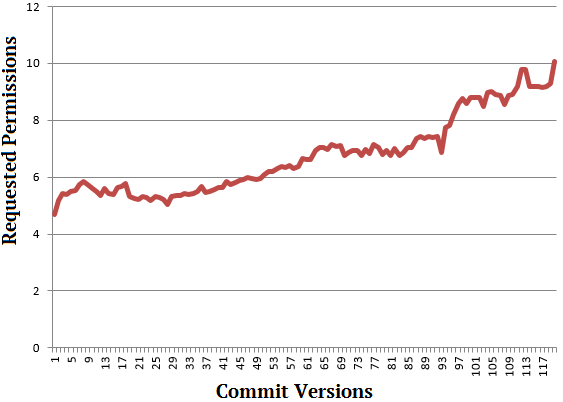
\includegraphics[width=\linewidth]{images/PermissionLifeCycle.png}
              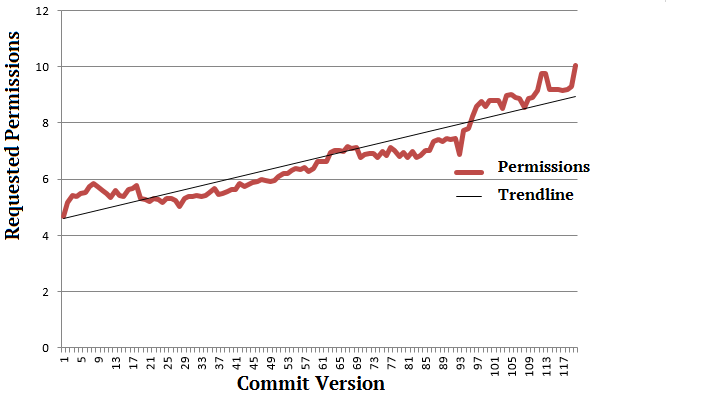
\includegraphics[scale=0.55]{images/PermissionLifeCycleTrendLine.png}

              \caption{Rate of Added Permissions}
              \label{fig:Evolution}
          \end{figure}
 %     \end{minipage}



On average, apps began with 4.68 permissions in their initial commit, and grew to requesting 10.05 permissions in commit 120. Our findings demonstrate that requested permissions are growing at a reasonably steady rate throughout an app's life cycle. Permissions change with every new Android API release and the number of available permissions has steadily grown since Android's inception. However, the rate of permissions being added to apps seems to far outpace the rate that new Android permissions are being created~\cite{AndroidSystemPermissions_URL}.

\noindent
\textbf{Analysis: }
These results indicate that permission-related decisions are made at a fairly steady rate throughout the development of the project, which demonstrates the need for developers to be constantly vigilant about properly using permissions. As with other types of functional and security testing, proper permission usage needs to be consistently checked throughout the development of an app.

%%% How does developer DCR score change over the lifecycle of the app? Do developers with higher DCR scores make more changes early or later?
%%%


%\dan{add to this}


%With the introduction of Android `M', users may be prompted for accept permission usage at runtime, and not only at install time as with previous versions of Android. \todo{why does this matter?}


% Ideas
% 	Developers need to pay constant attention to permissions
%	There is no single time when all permissions decisions are made
%	? How does this tie into overprivs?	
%	App permission growth will continue.
%	




% Add a "moving average bar" to the table - In excel this is called a "Trendline" ?
% The first 120 commits of apps with at least 120 alterations to their AndroidManifest file.


%%% Removed since I did not feel like an analysis would be all that useful
 % Surprisingly, there is a large jump in the number of requested permissions beginning from the \#94-\#120 commit mark with an average of 3.18 permissions added during this time frame. This is surprising since in the previous 93 commits, there was only an average growth of 2.19 permissions. % Our results also demonstrate that permissions are sometimes even removed from apps, which demonstrate that this is something which developers are paying attention to.

%The intent is to show that permissions are added at a near-linear rate, some limitations would include the availability of new permissions, or changes to the Android permission structure.




%%%%%%%%%%
% Look at committers across projects
% permission churn rate to permission usage
%



%\section{Ad Libraries} % Rename
%
%
%
%-	\hl{How often are AD libraries changed during the development process? When are they added during the app development process.}
%%		Where would these AD libraries be referenced? (In the code)?
%%		Could we build a detection mechanism to find these?
%%		Run PScout on the completed APK files. Get these values to see if there is a correlation.
%%	


% ? How does Android M work with Ad libraries? How does this new process affect things?

% Is there a correlation between Ad libraries, and permissions in general?
% Correlation between # of ads and rating (tie into mei's study)
% Correlation between when an ad is added (and number of them) and rating
% Do the commit messages tell us anything


% Maybe correlate with Findbugs: Have Cesar run Findbugs on the APKs and add these to the DB

% Look at Mei's Ad library paper to see how he discovered Ad libraries. This will likely be a larger, student driven task.



\section{Public Data Set \& Tool}
\label{sec: publicdata}


We have shared our primary discoveries, data, and all created software for this study on our project website at: \newline \textbf{http://www.Hidden.com}.

\subsection{Data}

Our data set contains all raw and processed project data including all extracted \emph{AndroidManifest.xml} files, version control information, permission changes and permission history. An overview of some of the publicly accessible data is shown in Table~\ref{Table:publicdata}. All data is available for external use and is available in an SQLite database.


 %	Total Projects: 1,179
 %	AndroidManifestFiles: 26,450
 %	PermissionChanges: 35,769
 %			A=17997
 %			R=17772
 %	Total project commits: 435, 680


 \begin{table}[h]
\begin{center}
\caption{Overview of Public Data Set}
\label{Table:publicdata}
 \begin{tabular}{ | l | c | } \hline

    \bfseries Value & \bfseries Count  \\ \hline \hline
    Total Projects & 1,179 \\ \hline
    Android Manifest files &  26,450 \\ \hline
    Permission Changes & 35,769 \\ \hline
    Total project commits & 435, 680 \\ \hline



  \end{tabular}
  \end{center}
\end{table}



This website not only contains the raw and processed project data, but also contains a suite of web based tools that other researchers may use in their work including the ability to query the data set on the web, and several customizable and pre-built reports.




%%%% Removed for space and because I didn't feel like it was all that useful. Add back in if space is not an issue.
%For example, Figure~\ref{fig:query1} demonstrates how users may query our data right on our webpage. We have chosen to make all of our data available not only for transparency, but for others to use in their own research as well.
%
%% talk about how Osara was made public
%
%
%% Show some images of the dataset
%
%
%% 	Show ability to query our data
%% 	Explore invidiual app information
%%	All manifest files and their data is also available on the project site
%
%
%
%          \begin{figure}[h]
%              %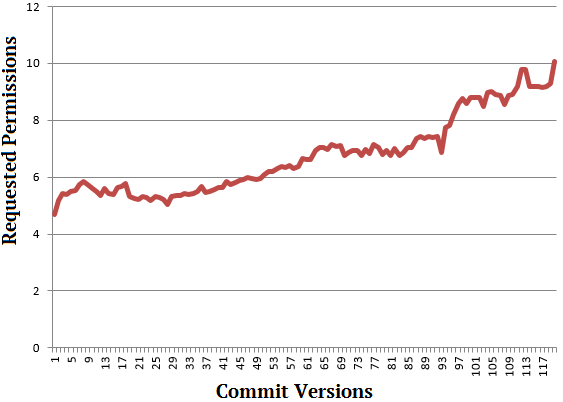
\includegraphics[width=\linewidth]{images/PermissionLifeCycle.png}
%              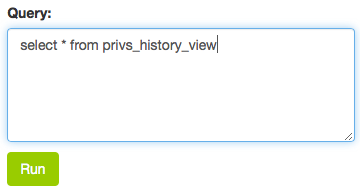
\includegraphics[scale=0.55]{images/privs_history_view.png}
%
%              \caption{Ability to Query Public Data Set}
%              \label{fig:query1}
%          \end{figure}







 \subsection{oSARA Tool}

We created Open Source Android Repository Analyzer (oSARA), to assist with crucial data extraction and analysis for this project. oSARA begins by extracting commit information from the collected git repository including who the committer was, when the commit was made, and the commit message. The tool then extracts all committed AndroidManifest.xml files from the version control history and records all modified permissions in these files. Using thise collected information, oSARA then determines all altered permissions, who made the alterations, and when they were made.

This tool and relevant documentation is available in a public version control system which is available on our project website. We encourage others to use this tool to not only replicate our study, but to build upon it to conduct their own research as well.

%this tool, we extracted version control commit information such
%as when the commit was made and who the committer was. The
%committed version of the AndroidManifest.xml file was also ex-
%tracted from from the repositories, and all metadata was stored in
%an SQLite database. Using this information, we were able to cor-
%relate the altered Android permissions with a specific commit in
%the version control repository. We then calculated the Developer?s
%Commit Ratio (DCR) for each app, which is defined as:

%% Available on our main project page

\vspace{7mm}
%%% Maybe provide a short section on this after each part?
\section{Limitations \& Future Work}
\label{sec: futurework}


% Future work
Although our results provided several interesting findings, there are areas which can be more thoroughly explored and elaborated upon. In our analysis, we studied open source Android apps in a variety of categories, but only from a single source (F-Droid). In future work, we will expand our app selection and include apps collected from other sources as well. However, this could be difficult since finding a substantial number of other open source repositories for Android apps may be a challenging process.


Previous work has analyzed apps through the examination of version control repositories and many studies have integrated developer interviews in their analysis. Our work should be expanded to include more developer interviews and more qualitative information. Further work could also be done to examine apps at different development stages using various static analysis tools  to examine a variety of security and quality based metrics of each app. Some potential tools include Stowaway~\cite{Felt:2011:APD:2046707.2046779}, PScout~\cite{Au:2012:PAA:2382196.2382222}, FindBugs~\cite{findbugs_key}, or TaintDroid~\cite{Enck:2010:TIT:1924943.1924971}


%%% Does DCR have an effect on permission misuse (probably briefly describe what permissions misuse is)
Android apps often suffer from permissions-misuse where apps often request too few, or too many permissions~\cite{Grace:2012:UEA:2185448.2185464, Felt:2011:APD:2046707.2046779}. Future work may be done to analyze if the DCR score of an permission has a higher rate of being misused. This analysis may be conducted using a permissions analysis tool such as PScout~\cite{Au:2012:PAA:2382196.2382222}. Future work could be conducted to determine if more mature apps, ones who have had longer version histories, tend to have high rates of permission misuse in comparison to new apps. Research may also be conducted to determine at what phases under and over-privileges are being added to apps.

%\todo{mention other 3rd party website}

We looked for a correlation between who made permissions based app alterations and the app's user rating. This may be an imprecise correlation since evaluating apps through user ratings is a difficult task as there are numerous security and quality metrics which may affect a user's perception of the app. Some studies have found that permissions significantly affect a user's perception of an app~\cite{Lin:2012:EPU:2370216.2370290}, while other studies have demonstrated that permissions play a much more insignificant role in a user's perception of an app and that there are numerous other factors which play a much more significant role~\cite{Kelley:2012:CPI:2426020.2426027, Felt:2012:APU:2335356.2335360}.


%% Look for users across different projects. Experts?
%% Correlate the size of the project into the analysis.


\section{Conclusion}
\label{sec: conclusion}


%The goal of this research was to better understand how permissions are being added to Android apps.


\noindent \textbf{Summary}:
We examined 1,179 open source Android apps from the F-Droid repository to better understand when, why and how permissions are added to open source Android apps. We also checked for a correlation between the number of permissions and total app commits by a developer, and user ratings.

\noindent \textbf{Findings}:
We found that: I) Developers with a low number of project based commits make a disproportionately high number of permissions-related commits. II) The user rating of an app is not affected by the number of permissions added by low or high-committers. III) Permissions are added at a reasonably consistent rate to an app during its development.

%\todo{update all of this}

%We found that: A) There is only a very weak correlation in the ratio of permissions based commits and overall project commits by a developer. In fact, we found that developers with low overall project commits make a disproportionately high number of permissions related commits. B) That there is no significance correlation in the ratio of permission based commits to overall project commits of a developer, and user rating of the app. C) Permissions are
%added at a fairly consistent amount throughout the software project. \todo{reword this entire section}

\newpage
\balance

\bibliographystyle{abbrv}
\bibliography{FdroidPermissions}



\end{document}



%%%%

%   Submission info
%   https://www.softconf.com/h/sac2017/cgi-bin/scmd.cgi?scmd=aLogin&passcode=1167X-G5H6F5F5B6
%     (withdrawn)


% Todo
%   Fix the format of the paper
%   Remove reference counter






















%*********
%	- Re-examine the top 10% and bottom % overprivs


%*********



%%%%% Types of comparisions that we can do

%	Kolmogorov-Smirnov
%	Mann-Whitney U
%	Standard deviation




%? Who is removing the overprivs
%-- double check the results to make sure that they are accurate
%
%
%- Are developers that change permissions more often more likely to add overprivs?
%
%********
%We next checked to see
%
%
%
%-- For all developers, see if there is a correlation with the number of added permissions and recorded overprivs
%
%
%
%
%
%-- If people add 1 overpriv, are they likely to add another?
%-- Are the same people adding overprivs, removing them?
%-- How frequently are overprivs removed?

%%% Todo



%%% Other stats ideas
% 	Interview some of Hussein's friends. See if we can do a developer study.
%		Potential questions: Who adds permissions to apps? When are they added? Why do you add or remove permissions from apps? How much attention do you pay to app permissions?
%	? Has this type of study been done before?



% Other RQs
%	







%%% Other random thoughts
%	Who is adding the overprivs
%	Are people removing the overprivs
%	When are they being added in
%	What is the rate of adding and removing permissions

% What permissions are most likely to be added, but not altered. Does this tie into permission comprehension.


%% Actions
%	Double check the results being returned from the manifest examination list
%	How many apps have Android M. Would I be able to get enough good results from this?


%%%%% Thoughts %%%%%
%   How long has a developer been with the project
%   Are permission decisions made in groups (do a scatter plot)
%   What do permission change comments indicate?
%   What else is changed along with permissions? - Related functionality
%   Who is adding the "dangerous" permissions vs the regular ones?
%



%	What motivates you to add or remove permissions to an app (text)?
%	How comfortable do you need to feel with a project before you modify its permissions? (likert)
%	How confident do you feel removing another developer's permissions, even if you feel like they are unnecessary? (likert)
%	Do you feel like the permissions process in projects (adding and removing permissions) generally does well (likert)?
%	What are the most significant permission related problems you encounter when working on projects with others? (text) - reword
%	How much does knowing the app better help you to most appropriately select the correct permissions for the app (likert)?
%	




%Make sure that these are good research questions to be asking before I go and do them

% Check to see who is adding ads to an app
%	How to find out when an ad is added to a repo
%	Check to see if ads and permission changes are occurring on the same commit
%			? Why would this be an issue?
% 	? What existing tools detect the precense of an ad library? Where does this generally go? The Manifest file?

% ? Can we use M-Perm to find overprivs




%% Thoughts 9/30/16 *****************
%   Are permissions with low DCR scores more likely to be changed later on? These changes could represent errors


%%%% Do an analysis of the liklihood that permissions would be removed from the system. Who added them.

% One method of determining whether or not a permission was appropriate to be added to a system is if the permission was removed.



% Threat: Permissions may be removed for a variety of reasons including requirments or API changes. Permissions are not always removed due to them being incorrect.


% 1) Do I need to do this?
% 2) What is the best way to do this?


% Get a list of all removed permissions (maybe also compare to a list of added permissions)
% High and low ranking commits. See if there a statistical differnce.



%%%% Query to get a list of all added/removed permissions and who changed them (DCR scores)



%%%% More ideas:

% Run against PScout to see who is creating over and under privs
% 


select *
from PermissionAdderInfo pai
inner join CommitterPercentage_view cv on pai.AppName = cv.AppName and cv.trimmedEmail = AuthorEmail




